\chapter{Verification} \label{chap:verification}
This chapter will focus on description and verification of ORB-SLAM2 \cite{murORB2} improved solution proposed in IROS 2019 conference \cite{iros2019}. Primary it will describe how ORB-SLAM2 works. Secondly it will show an accurate inspection necessary to find some potential bugs that cause an unexpected behaviour of the algorithm in a sequential environment.

 \section{System description}
 As described in \cite{iros2019}, ORB-SLAM2 is a Simultaneous Localization And Mapping system that can works with data coming from monocular, stereo, and RGB-D cameras. A system of this kind has the purpose to allow both map reconstruction and navigation in the most common environment without the support of a GPS.
 The system consists of the following three main blocks (see figure \ref{fig:orbslam}):

\begin{description}
	\item[Tracking and localization] 
	This block is in charge of computing visual features, localizing the robot in the environment, and, in case of significant discrepancies between an already saved map and the input stream, communicating updated map information to the mapping block. The frames per second (FPS) that can be computed by the whole system strongly depends on the performance of this block.
	\item[Mapping] 
	It updates the environment map by using the information (map changes) sent by the localization block. It is a computational time consuming block and its execution rate strictly depends on the agent speed. However, considering the actual agent speed of the KITTI datasets analysed in this work \cite{CVPR2012}, it does not represent a system bottleneck.
	\item[Loop closing] 
	It aims at adjusting the scale drift error accumulated during the input analysis. When a loop in the robot pathway is detected, this block updates the mapped information through a high latency heavy computation, during which the first two blocks are suspended. This can lead the robot to loose tracking and localization information and, as a consequence, the robot to get temporary lost. The computation efficiency of this block (running on-demand) is crucial for the quality of the final results.
\end{description}

\begin{figure}
	\centering
	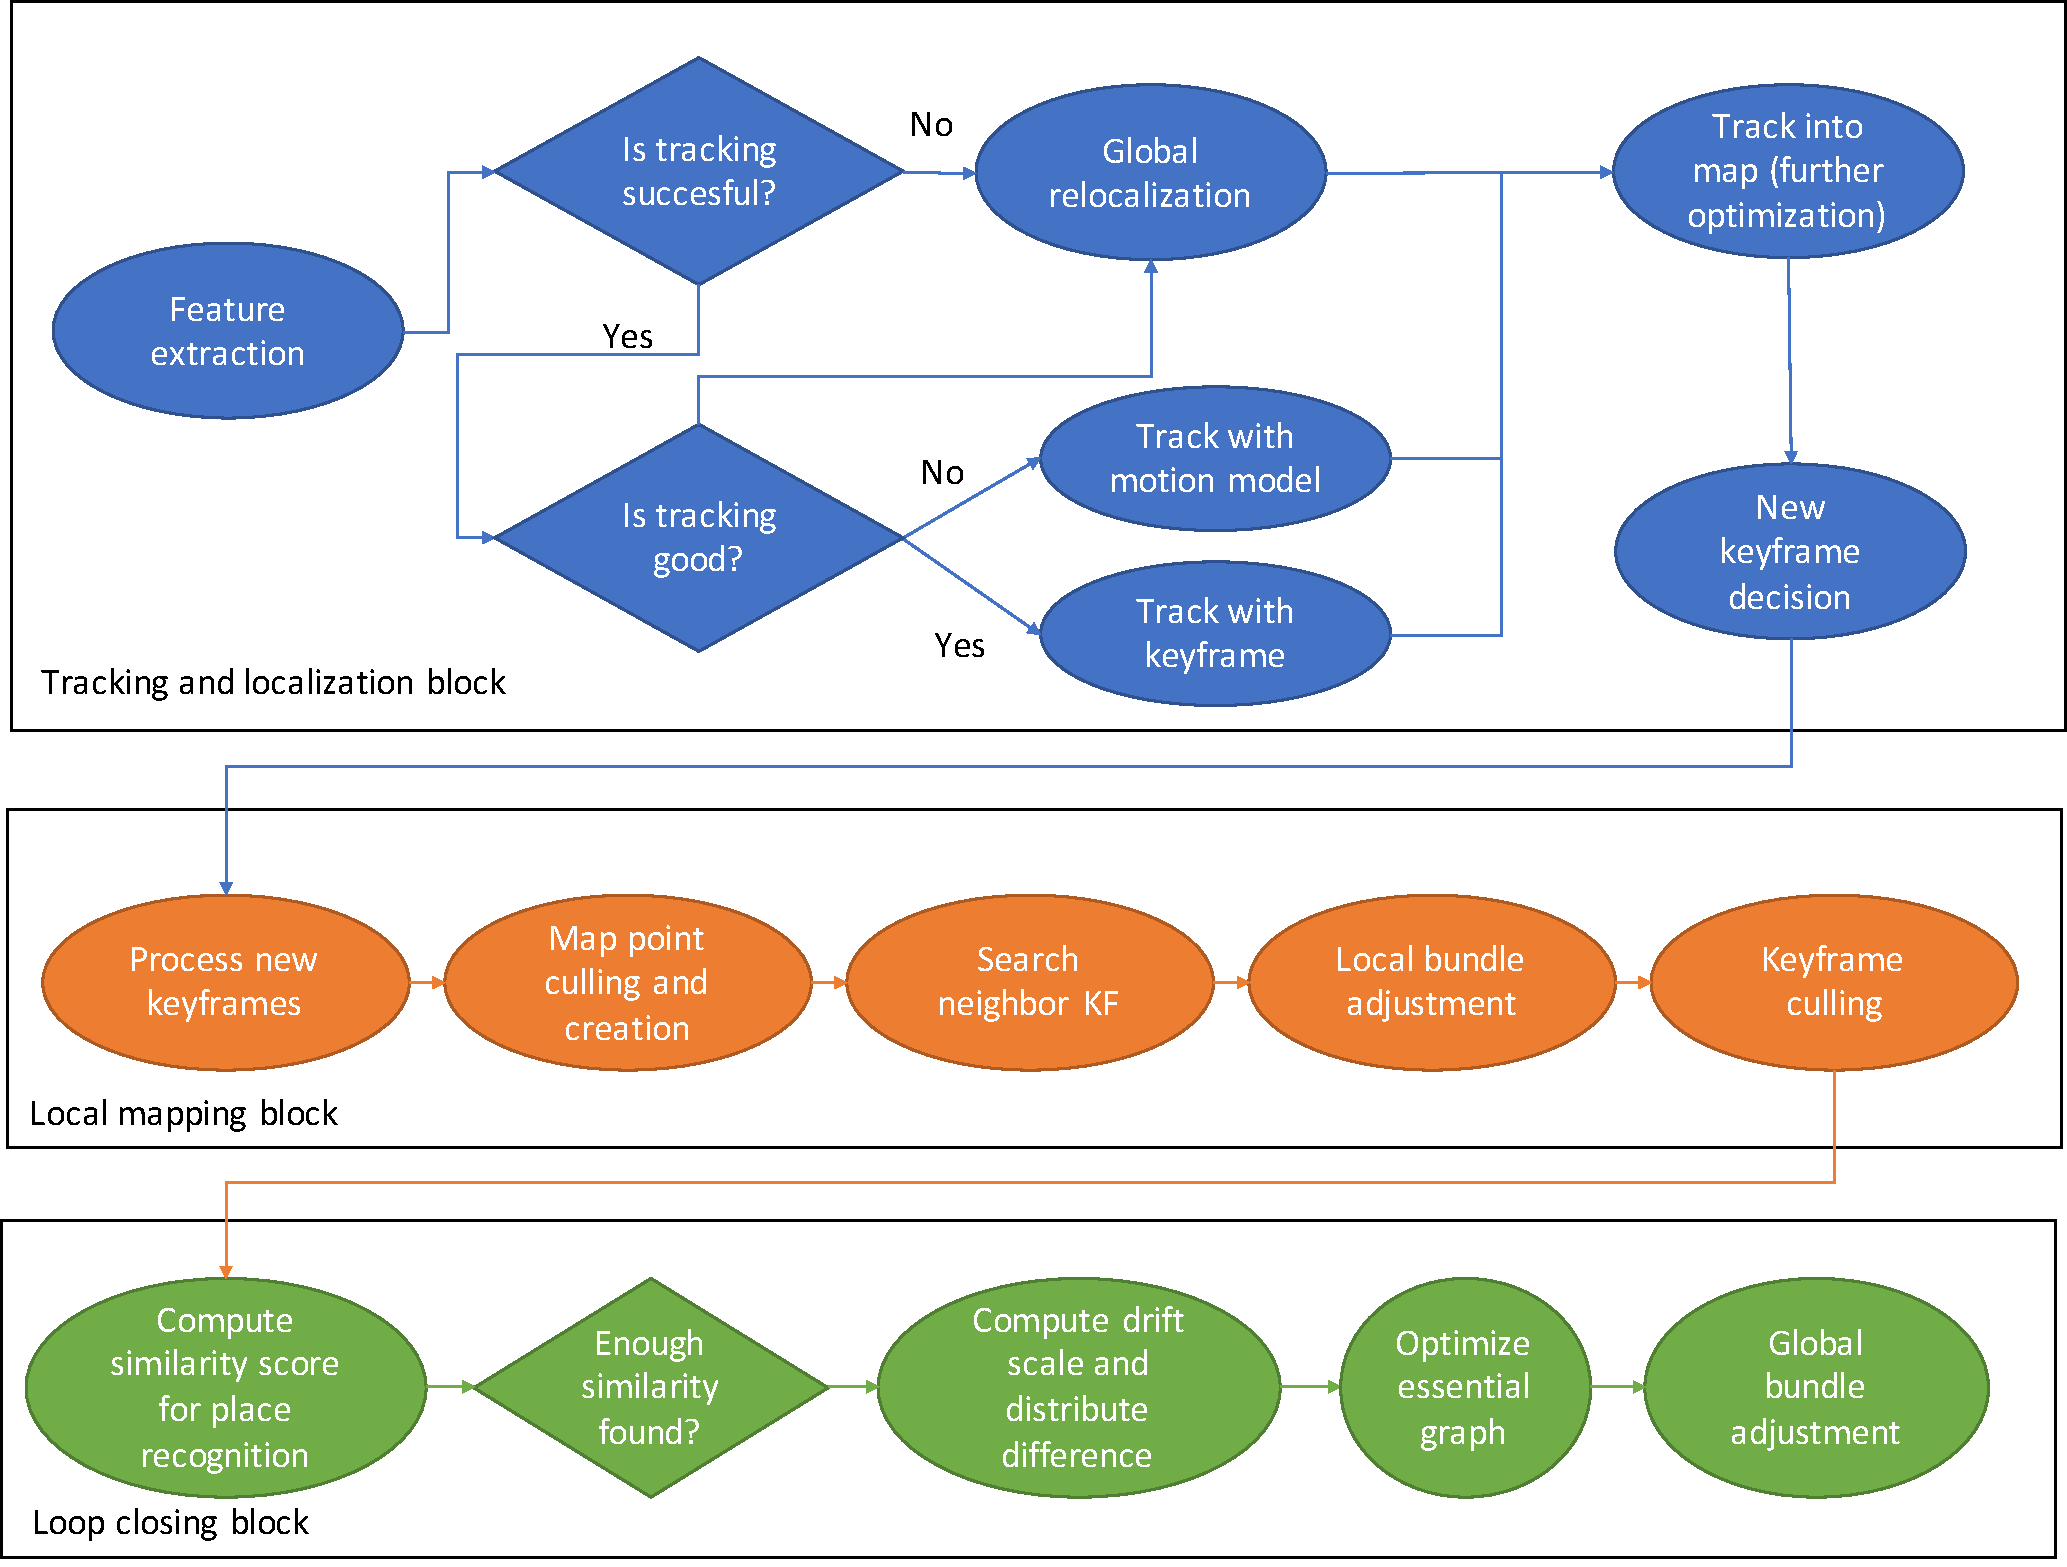
\includegraphics[width=\textwidth]{images/orb-slam-overview}
	\caption{Main blocks of the ORB-SLAM2 algorithm.}
	\label{fig:orbslam}
\end{figure}

The system is organized on three parallel threads, one per block. The use of parallel threads allows for obtaining real-time processing on an Intel Core i7 desktop PC with 16GB RAM \cite{murORB2}.


\section{Unexpected behaviour}

\subsection{The problem of the non-determinism} % possible reasons that cause a non deterministic behaviour


\subsection{The problem of the concurrency} % when we setup the orbslam to run sequentially it works worse that when it run concurrently.




\section{Discussion}
In this chapter the problem of non deterministic behaviour has been addressed and some of the possible solutions to overcome the problem of ...  have been presented.

The strategy adopted to achieve the goal of ... could reduce the ... in the system.


\clearpage
\thispagestyle{empty}